\chapter{Geometry Tools Needed to Study Trigonometry}
\label{chap:geometry_tools_needed_to_study_trigonometry}

\section{Right Triangles}
\label{sec:right_triangles}

There are three main types of angles:

\begin{itemize}
	\label{item:three_main_types_of_angles}

	\item Acute Angles
	\item Right Angles
	\item Obtuse Angles
\end{itemize}

\begin{definition}[Angles]
	\label{def:angles}$ $

	An \textbf{acute angle} is an angle with a measure less than $90^{\circ}$.

	An \textbf{right angle} is an angle with a measure of $90^{\circ}$.

	An \textbf{obtuse angle} is an angle with a measure greater than
	$90^{\circ}$.
\end{definition}

Recall from geometry that you need three known measures to describe a triangle
-- the lengths of two sides and the measure of an angle, the lengths of three
sides, or three other measures. For a right triangle, you need only two
additional measures, because you already know that one of the angles' measure
is $90^{\circ}$.

The following four cases describe all possible ways to describe a right triangle:

\begin{enumerate}
	\label{enum:four_ways_to_describe_a_right_triangle}

	\item The lengths of two legs
	\item The lengths of one leg and the hypotenuse
	\item The lengths of one leg and the measure of an acute angle
	\item The length of the hypotenuse and the measure of one acute angle
\end{enumerate}

Suppose you need to calculate the lengths of all three sides. For cases $1$ and
$2$, you only need geometry, specifically, the Pythagorean Theorem. But for
cases $3$ and $4$, you need trig to get the remaining sides.

\subsection{The Pythagorean Theorem}
\label{sub_sec:the_pythagorean_theorem}

Let's take a look at the famous geometry tool \textit{Pythagorean Theorem},
which helps us solve for cases $1$ and $2$.

\begin{theorem}[Pythagorean Theorem]
	\label{thrm:pythagorean_theorem}

	The \textbf{Pythagorean Theorem} states that if $a$ and $b$ are the lengths
	of the legs of a right triangle and $c$ is the length of the hypotenuse,
	then:

	\[ a^{2} + b^{2} = c^{2} . \]
\end{theorem}

\begin{exc}
	Let's illustrate how cases $1$ and $2$ can be solved with the help of the
	Pythagorean Theorem.

	Two legs of a right triangle measure $5$ and $12$ inches. Find the hypotenuse.

	\begin{figure}[H]
		\centering

		\begin{tikzpicture}
			\coordinate [label=above:$A$] (A) at (0,2);
			\coordinate [label=right:$B$] (B) at (4,0);
			\coordinate [label=left:$C$] (C) at (0,0);

			\draw (C) -- node[below] {$4$} (B) -- node[above] {$5$} (A) -- (C);
		\end{tikzpicture}

		\label{fig:right_triangle_with_5_inch_and_12_inch}
	\end{figure}

	Since you know the length of the two legs, you can substitute those into the
	theorem's equation:

	\begin{align*}
		a^{2} + b^{2}  & = c^{2} \\
		5^{2} + 12^{2} & = c^{2} \\
		25 + 144       & = c^{2} \\
		169            & = c^{2} \\
		\sqrt{169}     & = c     \\
		c              & = 13
		.\end{align*}

	\solution

	The length of the hypotenuse is $13$ inches long.
\end{exc}

% subsection the_pythagorean_theorem (end)

\subsection{Special Right Triangles}
\label{sub_sec:special_right_triangles}

In this section, we'll take a look at two special kinds of right triangles. For
these special triangles, if you know the length of any one side of the
triangle, you can find the length of the other two sides.

\begin{figure}[htpb]
	\centering

	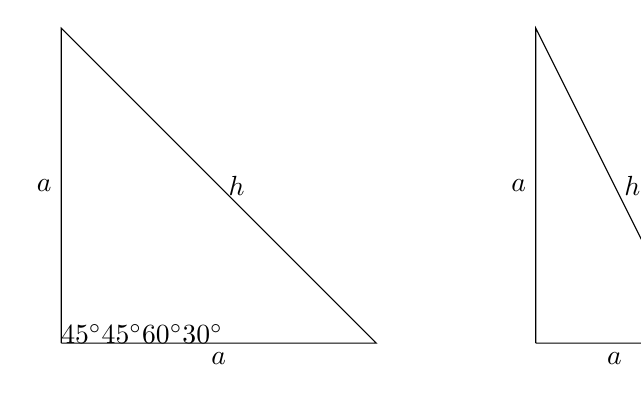
\begin{tikzpicture}
		\coordinate (A) at (0,4);
		\coordinate (B) at (4,0);
		\coordinate (C) at (0,0);

		\draw (C) -- node[below] {$a$} (B) -- node[right] {$h$} (A) -- node[left] {$a$} (C);

		\tkzMarkAngle[size=0.5cm](A,B,C)
		\tkzMarkAngle[size=0.5cm](C,A,B)

		\tkzLabelAngle(A,B,C){$45^{\circ}$};
		\tkzLabelAngle(C,A,B){$45^{\circ}$};

		\coordinate (A) at (5,4);
		\coordinate (B) at (7,0);
		\coordinate (C) at (5,0);

		\draw (C) -- node[below] {$a$} (B) -- node[right] {$h$} (A) -- node[left] {$a$} (C);

		\tkzMarkAngle[size=0.5cm](A,B,C);
		\tkzMarkAngle[size=0.5cm](C,A,B);

		\tkzLabelAngle(A,B,C){$60^{\circ}$};
		\tkzLabelAngle(C,A,B){$30^{\circ}$};
	\end{tikzpicture}

	\label{fig:45_45_90_and_30_60_90_triangle}
\end{figure}

The triangle on the left is called a $45^{\circ}-45^{\circ}-90^{\circ}$
triangle, or an isosceles right triangle. The triangle on the right is called a
$30^{\circ}-60^{\circ}-90^{\circ}$ triangle. The Pythagorean Theorem is used to
prove the following relationship that exist in these two special right
triangles.

\begin{definition}[Isosceles Right Triangle]
	\label{def:isosceles_right_triangle}

	An \textbf{isosceles right triangle} is a triangle that has two equal sides
	and two equal angles, as well as a third angle that is a right angle. The
	only triangle that satisfies all these conditions is a
	$45^{\circ}-45^{\circ}-90^{\circ}$ triangle.
\end{definition}

\begin{theorem}
	If each acute angle of a right triangle measures $45^{\circ}$, the hypotenuse
	is $\sqrt{2}$ times as long as a leg.

	\begin{figure}[H]
		\centering

		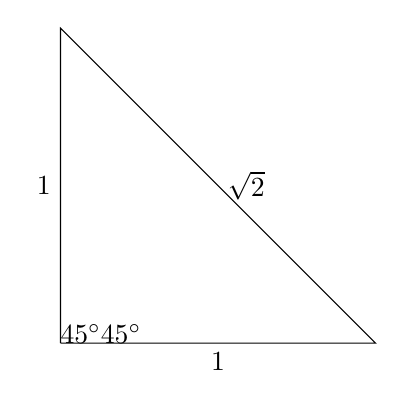
\begin{tikzpicture}
			\coordinate (A) at (0,4);
			\coordinate (B) at (4,0);
			\coordinate (C) at (0,0);

			\draw (C) -- node[below] {$1$} (B) -- node[right] {$\sqrt{2}$} (A) -- node[left] {$1$} (C);

			\tkzMarkAngle[size=0.5cm](A,B,C)
			\tkzMarkAngle[size=0.5cm](C,A,B)

			\tkzLabelAngle(A,B,C){$45^{\circ}$};
			\tkzLabelAngle(C,A,B){$45^{\circ}$};
		\end{tikzpicture}

		\label{fig:45_45_90_triangle}
	\end{figure}
\end{theorem}

\begin{example}
	If one leg in a $45^{\circ}-45^{\circ}-90^{\circ}$ triangle is $10$ units
	long, then the hypotenuse is $10\sqrt{2}$ units long.
\end{example}

\begin{theorem}
	If acute angles of a right triangle measure $30^{\circ}$ and $60^{\circ}$,
	then the hypotenuse is twice as long as the shortest leg and the longer leg
	is $\sqrt{3}$ times as long as the shortest leg.

	\begin{figure}[H]
		\centering

		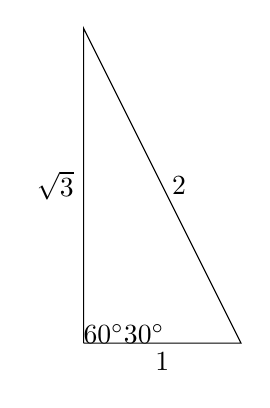
\begin{tikzpicture}
			\coordinate (A) at (0,4);
			\coordinate (B) at (2,0);
			\coordinate (C) at (0,0);

			\draw (C) -- node[below] {$1$} (B) -- node[right] {$2$} (A) -- node[left] {$\sqrt{3}$} (C);

			\tkzMarkAngle[size=0.5cm](A,B,C);
			\tkzMarkAngle[size=0.5cm](C,A,B);

			\tkzLabelAngle(A,B,C){$60^{\circ}$};
			\tkzLabelAngle(C,A,B){$30^{\circ}$};
		\end{tikzpicture}

		\label{fig:30_60_90_triangle}
	\end{figure}
\end{theorem}

\begin{example}
	If the shortest leg in a $30^{\circ}-60^{\circ}-90^{\circ}$ triangle is $6$
	units long, then the hypotenuse is $2 \times 6 = 12$ units long, and the
	longest leg is $6\sqrt{3}$ units long.
\end{example}

% subsection special_right_triangles (end)

\subsection{Classifying Triangles}
\label{sub_sec:classifying_triangles}

Any triangle is six elements: three sides and three angles. Throughout this
book, I use capital letters ($A, B, C$) to denote measures of angles and
lowercase letters. I also use lowercase letters ($a, b, c$) to denote sides of
the triangles I use the small letter corresponding to the name of the angle
opposite to this side. I also use the symbol $\triangle$ to identity a
triangle. Therefore, an expression $\triangle ABC$ means "the triangle $ABC$".

\begin{figure}[htpb]
	\centering

	\begin{tikzpicture}
		\coordinate [label=above:$A$] (A) at (2,4);
		\coordinate [label=right:$C$] (B) at (4,0);
		\coordinate [label=left:$B$]  (C) at (0,0);

		\draw (C) -- node[below] {$a$} (B) -- node[right] {$b$} (A) -- node[left] {$c$} (C);
	\end{tikzpicture}

	\label{fig:generic_triangle}
\end{figure}

When given the lengths of three sides, you can construct a triangle that is
determined by these sides; therefore, its angles are determined as well.
However, you need to be careful thinking this way, because not all arbitrary
side lengths enable us to construct a triangle. Before constructing a triangle
given its sides, you need to refer to the \textit{Triangle Inequality}.

\begin{definition}[Triangle Inequality]
	\label{def:triangle_inequality}

	The \textbf{triangle inequality} states that the sum of the lengths of any
	two sides of a triangle is greater than the length of the third side.
\end{definition}

\begin{example}
	\label{exm:triangle_inequality}

	Let's state whether it's possible for a triangle to exist with sides of the
	given lengths:

	\textbf{Sample 1:} The given sides are $4$, $5$, and $6$ units long. You
	need to compare the sums of any two sides with the third side. That means
	you need to exhaust all possibilities:

	\begin{align*}
		4 + 5 & = 9 > 6  \\
		4 + 6 & = 10 > 5 \\
		5 + 6 & = 11 > 4
		.\end{align*}

	\textbf{Sample 2:} The given sides are $1$, $2$, and $3$ units long. Let's
	try all possibilities:

	\begin{align*}
		2 + 3 = 5 > 1 \\
		3 + 1 = 4 > 2 \\
		1 + 2 = 3 = 3
		.\end{align*}

	The sum of these two sides ($1$ and $2$) are not greater than the third side
	($3$). Therefore, this triangle doesn't exist.
\end{example}

A triangle can be classified as acute (having three acute angles), right
(having one right angle), and obtuse (having one obtuse angle). As we
discussed, the lengths of the sides of a triangle determine its angles. Given
the lengths of the sides, can you tell whether the triangle is acute, right, or
obtuse?

The pythagorean theorem gives us a partial answer. We know that if the lengths
satisfy the relationship $a^{2} + b^{2} = c^{2}$, then we know it's a right
triangle. If it doesn't, then it's either an acute or obtuse triangle.

\begin{align*}
	\textrm{If } \angle C \textrm{ of } \triangle ABC \textrm{ is acute, then } c^{2} < a^{2} + b^{2} \\
	\textrm{If } \angle C \textrm{ of } \triangle ABC \textrm{ is obtuse, then } c^{2} > a^{2} + b^{2}
	.\end{align*}

Using this information and given the sides' lengths, you can identify the type
of triangle you are dealing with.

\begin{example}
	\label{exm:type_of_triangle}

	If the sides are $6$, $7$, $8$, by substituting those values, you get:

	\[ 8^{2} = 64 < 6^{2} + 7^{2} = 36 + 49 = 85 . \]

	So, this triangle is an acute triangle.
\end{example}

\begin{note}
	\label{not:which_number_is_the_hypotenuse}

	In a triangle, the hypotenuse is always bigger in length than either of the
	sides. Hence, we always know which number should be substituted for $c$ since
	it's the largest one of the three.

	If the sides are $6$, $8$, and $10$, then:

	\[ 10^{2} = 100 = 6^{2} + 8^{2} = 36 + 64 = 100 . \]

	So the triangle is a right triangle.

	If the sides are $5$, $12$, and $14$, then:

	\[ 14^{2} = 196 > 5^{2} + 12^{2} = 25 + 144 = 169 . \]

	So the triangle is an obtuse triangle.
\end{note}

% subsection classifying_triangles (end)

% section right_triangles (end)

\section{Circles, Arcs, and Chords}
\label{sec:circles_arcs_and_chords}

Another basic shape talked about in geometry is a circle. Let's review some
basic elements of a circle because you use them a lot throughout trigonometry.

\subsection{Chords and Arcs}
\label{sub_sec:chords_and_arcs}

Let's analyze the circle below and take note of its key elements.
$\overline{OA}$ is a radius. $\overline{RS}$ is a chord. $\overline{BC}$ is a
diameter.

\newpage

\begin{figure}[htpb]
	\centering

	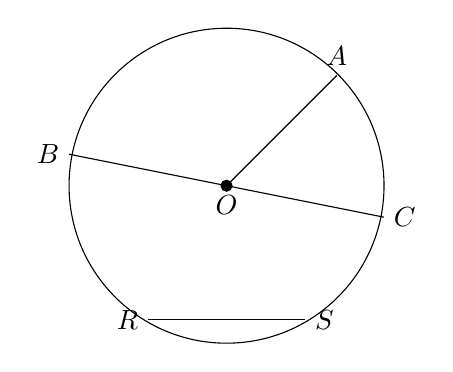
\begin{tikzpicture}
		\coordinate[label=below:$O$]  (O) at (0,0);
		\coordinate[label=above:$A$]  (A) at (1.4,1.4);
		\coordinate[label=left:$B$]   (B) at (-2,0.4);
		\coordinate[label=right:$C$]  (C) at (2,-0.4);
		\coordinate[label=left:$R$]   (R) at (-1,-1.7);
		\coordinate[label=right:$S$]  (S) at (1,-1.7);

		\draw[fill=black] (O) circle (0.07);

		\draw (O) circle (2);
		\draw (O) -- (A);
		\draw (B) -- (C);
		\draw (R) -- (S);
	\end{tikzpicture}

	\label{fig:circle_with_radius_chord_and_diameter}
\end{figure}

\begin{definition}[Radius]
	\label{def:radius}

	A \textbf{radius} of a circle is a segment that joins the center of a circle
	to a point on the circle.
\end{definition}

\begin{definition}[Chord]
	\label{def:chord}

	A \textbf{chord} is a straight line segment joining two points that lie on
	the circumference of a circle. A chord whose endpoints lie opposite to each
	other on the circle and whose center passes through the circle's center is
	referred to as the diameter.
\end{definition}

\begin{definition}[Diameter]
	\label{def:diameter}

	A \textbf{diameter} is a chord that contains the center.
\end{definition}

Now, let's discuss central angles and arcs of a circle.

\begin{figure}[htpb]
	\centering

	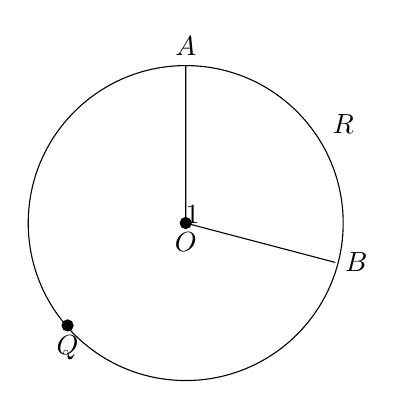
\begin{tikzpicture}
		\coordinate[label=below:$O$]  (O) at (0,0);
		\coordinate[label=above:$A$]  (A) at (0,2);
		\coordinate[label=right:$B$]  (B) at (1.9,-0.5);
		\coordinate[label=below:$Q$]  (Q) at (-1.5,-1.3);
		\coordinate[label=below:$R$]  (R) at (2,1.5);

		\draw[fill=black] (O) circle (0.07);

		\draw (O) circle (2);
		\draw (A) -- (O) -- (B);

		\draw[fill=black] (Q) circle (0.07);

		\tkzMarkAngle[size=0.5cm](B,O,A);
		\tkzLabelAngle(B,O,A){$1$};
	\end{tikzpicture}

	\label{fig:angles_and_arcs_of_a_circle}
\end{figure}

$\angle 1$ is the central angle of the circle $O$. $R$ is a minor arc between
the points $A$ and $B$, which is denoted as arc $AB$. The part that isn't
between points $A$ and $B$ are referred to as the major arc $AQB$.

\begin{note}
	To name a major arc, three letters must be used.
\end{note}

The measure of a minor arc is defined to be the measure of its central angle.
If the measure of $\angle 1 = 40^{\circ}$, you can write the measure of $AB =
	40^{\circ}$ as well. The measure of a major arc is calculated by subtracting
$40^{\circ}$ from $360^{\circ}$:

\[ 360^{\circ} - 40^{\circ} = 320^{\circ} . \]

\begin{definition}[Central Angle]
	\label{def:central_angle}

	A \textbf{central angle} of a circle is an angle with a vertex at the center
	of the circle.
\end{definition}

\begin{definition}[Minor Arcj]
	\label{def:minor_arcj}

	A \textbf{minor arc} of a circle is the union of two points on the circle and
	all the points of the circle that lie on the interior of the central angle
	with sides that contain the two points. Minor arcs measure less than
	$180^{\circ}$.
\end{definition}

\begin{definition}[Major Arc]
	\label{def:major_arc}

	A \textbf{major arc} is an arc of a circle having measure greater than or
	equal to $180^{\circ}$.
\end{definition}

\begin{example}
	\label{exm:angles_and_arcs_of_a_circle}$ $

	\begin{figure}[H]
		\centering

		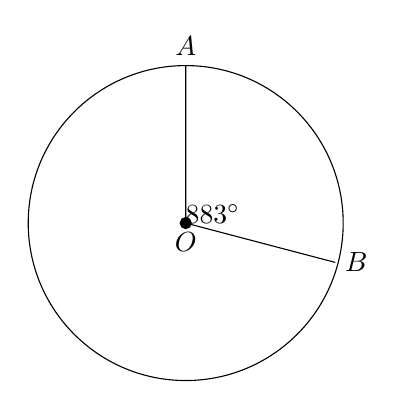
\begin{tikzpicture}
			\coordinate[label=below:$O$]  (O) at (0,0);
			\coordinate[label=above:$A$]  (A) at (0,2);
			\coordinate[label=right:$B$]  (B) at (1.9,-0.5);

			\draw[fill=black] (O) circle (0.07);

			\draw (O) circle (2);
			\draw (A) -- (O) -- (B);
			\tkzLabelSegment[left](A,O){$8$};

			\tkzMarkAngle[size=0.5cm](B,O,A);
			\tkzLabelAngle(B,O,A){$83^{\circ}$};
		\end{tikzpicture}

		\label{fig:angles_and_arcs_of_a_circle}
	\end{figure}

	In a circle of radius $8$, how long is the chord of an arc of $83^{\circ}$?
	It turns out again that geometry doesn't have the tools to solve this
	problem. This problem provides a glimpse of types of problems that
	trigonometry will help solve.
\end{example}

% subsection chords_and_arcs (end)

\subsection{Area of Circles}
\label{sub_sec:area_of_circles}

To find the area of a circle, you need to know its radius. You can then use the following formula to calculate its area.

\[ A = \pi r^{2} . \]

\begin{example}
	\label{exm:area_of_a_circle}

	If the radius is $7$ inches, the area of the circle can be calculated by
	substituting this value into the formula:

	\[ A = \pi r^{2} \implies \pi 7^{2} = 49\pi . \]
\end{example}

% subsection area_of_circles (end)

% section circles_arcs_and_chords (end)

% chapter geometry_tools_needed_to_study_trigonometry (end)

\newpage
